%!TEX root = ../template.tex
%%%%%%%%%%%%%%%%%%%%%%%%%%%%%%%%%%%%%%%%%%%%%%%%%%%%%%%%%%%%%%%%%%%%
%% benchmark.tex
%% NOVA thesis document file
%%
%% Chapter with a short latex tutorial and examples
%%%%%%%%%%%%%%%%%%%%%%%%%%%%%%%%%%%%%%%%%%%%%%%%%%%%%%%%%%%%%%%%%%%%

\typeout{NT FILE benchmark.tex}

\chapter{PouchBeasts: A Benchmark Application}
\label{cha:benchmark}

In this chapter, we present the third contribution from this dissertation, named ``PouchBeasts''. PouchBeasts consists in a benchmark application, for a back-end of an edge-enabled interactive multiplayer game, with functionality inspired by the popular game PokemonGO \cite{pokemonGo}. This contribution arose from the suggestion presented in \cite{Leitao2018}, and it aims to present a materialization of a benchmark with focus on real-time interactions between users. The importance of this contribution is its' possible use to test service deployment systems, given the user interactions can be dramatically influenced, in terms of quality of service, the proximity to the deployment of its' services (i.e. users performing real-time battles mediated by a server in a different continent will have a poor user experience).

% PouchBeasts was attained through the combined efforts with a colleague, with the goal of being a proof-of-concept for the realization of a fully decentralized resource management system, that uses DeMMon as the solution for managing the nodes in an overlay network, and monitoring the execution of the PouchBeasts microservices. Then, this monitoring information is used by a decentralized service deployment solution to optimize the services supporting the execution of ``PouchBeasts'' via geographical heuristics (the latter is my colleagues' work).

PouchBeasts was attained through the combined efforts with a colleague, with the goal of being a proof-of-concept for the realization of a fully decentralized resource management system. The intention is to use this benchmark with DeMMon as the solution for managing the nodes in an overlay network, and for monitoring the execution of the PouchBeasts microservices. Then, this monitoring information is used by a decentralized service deployment solution to optimize the services supporting the execution of ``PouchBeasts'', via geographical heuristics, the latter being our colleagues' work.

In this application, registered users own a set of beasts, which they can expand by catching more beasts in certain gepgraphical areas, or by acquiring new ones in a shop. Beasts are collectable items with different properties (such as attack value, health points, experience, among other properties) which may be used to both battle against other users (and their beasts) and join other users in a cooperative battle against a computer-controlled beast. During these battles, users must command their beasts to either attack or defend and can also use items on their beasts, which can have multiple effects, such as: reviving dead beasts, healing a certain amount of health of a beast, among other uses. These items may be traded with other users or acquired from a shop using coins, which in turn are acquired through microtransactions.

\subsection{Overview}

\begin{figure}[htbp]
    \centering
    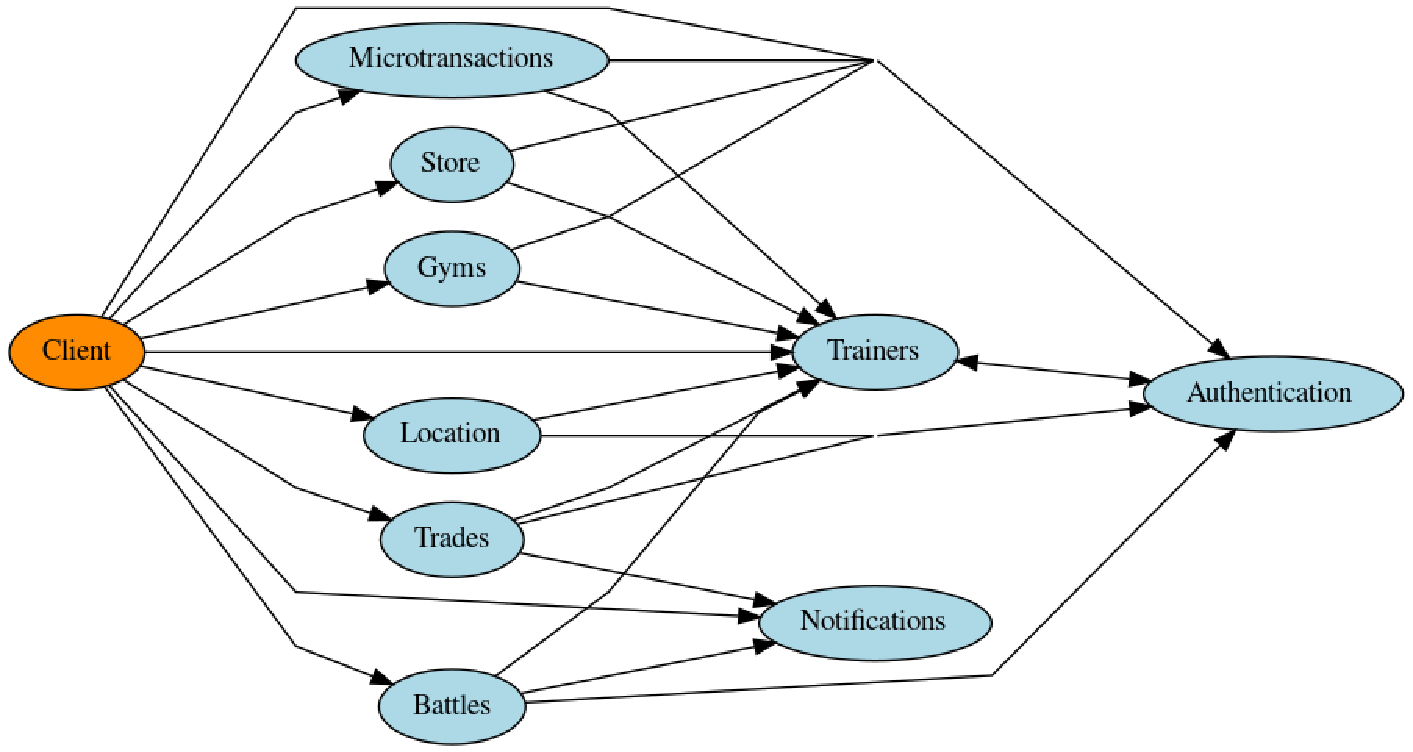
\includegraphics[width=\textwidth]{Chapters/benchmark/figures/interaction-diagram.pdf}
    \caption{An illustration of the dependencies between services of PouchBeasts}
    \label{fig:pouchbeasts-overview}
\end{figure}

The interactions between the services in this benchmark are illustrated in figure's \ref{fig:pouchbeasts-overview} diagram. There are nine microservices in total and a client to access them. We now provide a brief overview of each microservice and its role within the system:

\begin{enumerate}
    \item The first and most used microservice of the system is called \textbf{Trainers}, and it essentially stores all the data related to the users and their owned beasts. In addition, the service verifies the tokens issued by the Authentication microservice in regard to the recency of the information carried by the tokens. This service makes use of a MongoDB \cite{mongodb} database to store these records in permanent storage and to maintain data consistency across microservices.
    
    \item The next microservice is called \textbf{Authentication}, which only has the purpose of generating new authentication tokens for the users to use when interacting with other services. These tokens contain a hash of the owned beasts, so other servers can verify their authenticity and recency without having to fetch the users' beasts on each interaction.

    \item Following, we have the \textbf{Gyms} and \textbf{Battles} services and these allow players to perform combats with their obtained beasts. In the case of the Gym's service, it manages entities in the system denominated gymnasiums, which have a pre-assigned geographical location. In this service, if a user is within a geographical distance of a gymnasium, it may perform battles alongside other trainers against a single beast controlled by the computer. The \textbf{Battles} service is a service that allows users to use their beasts to perform battles against other users' beasts. Battles can either start via a queueing system, where players wait for another random user to start the battle, or by challenging other known users (via a notification). Whenever a user is in a battle, it issues commands (based on the observed battle status) and receives updates regarding the status of the battle. As commands depend on the observed status of the battle, it is paramount (for the quality of service of the users) that both the players' commands and the information passed from the battles/gyms service to the player suffer the least latency possible. The information regarding the issued commands and battle status is propagated to the user using WebSockets. Whenever a battle finishes, the Battles / Gyms server stores the battle result and update the users' beasts and items in the Trainers service.
    
    \item The \textbf{Store} and \textbf{Microtransactions} services provide ways for users to obtain currency via small value transactions, which can, in turn, be used in the store to buy new items. These items then have effects on the beasts (e.g. or reviving a dead beast or healing a beast which has little health).

    \item Users may also change their items via the \textbf{Trades} service. This service grants users the possibility to exchange their items with other users in the system. In order to use this system, a user must invite another currently active user via a notification (which can optionally be accepted by the target user). Whenever this notification is accepted, the two users connect to the server via a WebSockets connection and begin to submit the items they wish to trade. Whenever a player adds an item to the trade, this information is propagated by the server to the other player through a WebSockets connection. Whenever the users finish adding or removing items to the trade agreement, they accept the trade, and the Trades server commits the transaction result to the Trainers server.

    \item The service responsible for handling all of the previously mentioned notifications is called \textbf{Notifications}. This service is essentially tasked with receiving notifications from connected users and propagating them towards the target user. As there may be multiple Notification services executing concurrently and users may connect to any of the available servers, a notification may be emitted for a user not connected to the same server. To prevent these notifications from being lost, this service makes use of a Kafka \cite{apache_kafka} backend, which it uses to propagate messages targeting users that are connected to different notification servers.

    \item The last implemented microservice is called \textbf{Location} service, responsible for tracking the following entities contained within a geographical area: the geographical locations of users, the generation and management of the generated beasts (for users to catch), and the locations of gymnasiums. Essentially, location servers communicate with the users through a Websockets API, where users periodically receive locations of the nearby beasts and gyms. 
\end{enumerate}


In order to prevent multiple location services from managing overlapping geographical areas and to facilitate the insertion and decommission of new location servers, we assign portions of the geographical area to certain servers using S2 cells \cite{s2geometry}. S2 cells provide a framework for decomposing a sphere (in our case, the earth) into a hierarchy of cells, where each S2 cell is quadrilateral bounded by four geodesics. The top-level of the hierarchy is obtained by projecting the six faces (the topmost six cells) of a cube onto the earth, and lower levels are obtained by subdividing each cell into four children recursively. An example of two of the six face cells (one of which has been subdivided multiple times) can be observed in figure \ref{fig:pouchbeasts-s2cells}. This service makes use of S2 cells to (1) assign portions of the earth to servers in a way that does not create geographical discontinuities, (2) to index efficiently the locations of trainers, gyms and generated beasts, which allows the service to, based on the intersection of a cell centred on the user's location with the cells indexing the gyms and beasts, determine the set of beasts and gyms to return to emit to a certain user, (3) in the case a user's location is in the boundary of two (or more) location servers, S2 cells are also used to decide to which server(s) the user should connect. Similarly to before, this is also performed based on the intersection of a cell centred on the user's location with the cells indexing the gyms and beasts.

\begin{figure}[htbp]
    \centering
    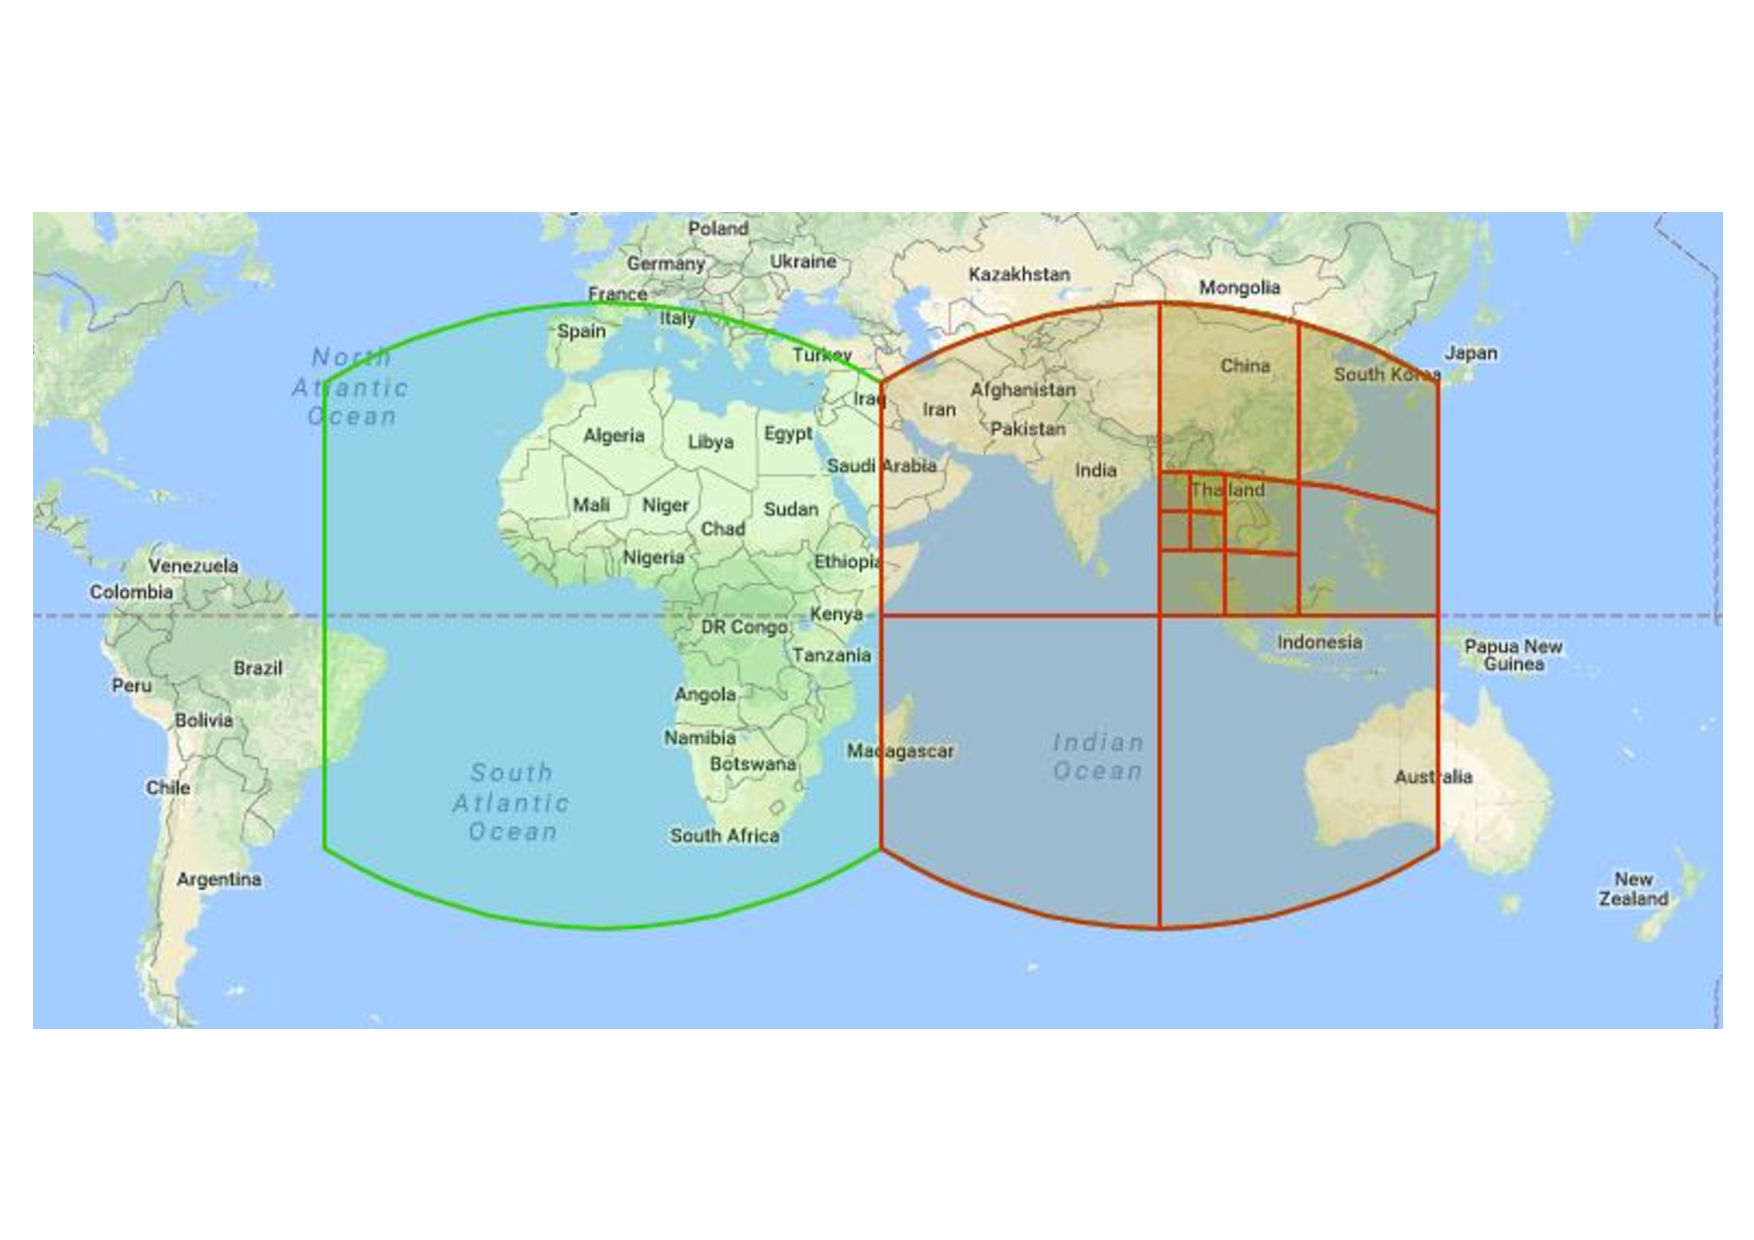
\includegraphics[width=\textwidth]{Chapters/benchmark/figures/s2_cells.pdf}
    \caption{Example of S2 cell hierarchy, taken from ``https://s2geometry.io/''}
    \label{fig:pouchbeasts-s2cells}
\end{figure}

Provided with the high-level overview of each of the implemented microservices of the benchmark, it is important to notice that the latency requirements regarding the interactions with the users and services are varied. For example, services such as the Trainers, Store or Microtransactions services are more tolerant when it comes to latency requirements when compared to services like the Gyms, Battles or Trades, as these have an interactive nature where a high latency value leads to frustration when it comes to user experience.

To test these interactions, the benchmark also contains a client which allows the execution of actions such as: battling other users, catching beasts, acquiring and spending tokens, among others. Then, through the instrumentation of both the client and the services, we provide metrics to quantify some aspects regarding these interactions, such as the delays in the interactions between users and servers in both Trades and Battles services, among other interactions. Provided with these indicators, then the performance of service deployment and maintenance systems can be assessed.

To enable automated client testing, we provide ways for clients to simulate user behavior. This is configurable via a configurable stochastic matrix, that contains a line and a row for each possible action to perform with the client, and each matrix position (given by a certain line and row) contains the probability of performing any of the other possible actions, provided the user just performed the action in the current line. 

Provided the objective of this benchmark is to test service deployment systems, we provide a deployment configuration of this benchmark for Kubernetes. With this baseline deployment system, commonly employed in the state-of-the-art, users who develop their service deployment systems have a baseline to compare to.

\subsection{Summary}

In this chapter, we covered the third contribution from this dissertation, named ``PouchBeasts''. This contribution, in the shape of a benchmark, aims to simplify the evaluation process of decentralized management and monitoring solutions, particularly those aimed at improving service deployments. It does so by providing both a client and a set of services (implemented by microservices) which offer a wide range of interaction types, from request-reply based interactions to real-time interactions, with varied demands in regard to server and client latency.

Although this benchmark was not employed to test the performance of DeMMon directly, it is important to mention that the previously mentioned colleague, that contributed the implementation of this benchmark has successfully built a system (for his dissertation) that, through the metrics obtained by the decentralized aggregation primitives provided by the DeMMon framework, improves the QoS of clients using the ``PouchBeasts'' services.